\documentclass[12pt, a4paper, pdflatex]{report}
%  notitlepage - abstract on the same page
\usepackage{indentfirst} % indent frst paragraph of section
% \usepackage{fullpage} % full A4 page
\usepackage[top=0.85in, bottom=1.44in, left=0.85in, right=0.85in]{geometry}
\usepackage{amsmath}
\usepackage[pdftex]{graphicx}
\usepackage{cite} % BiTeX
\usepackage{lipsum}
\newcommand{\ts}{\textsuperscript}
\usepackage[usenames,dvipsnames]{color}
\usepackage{pdfpages} % appending pdf file to tex document
\usepackage{url}
\usepackage{newclude} % include latex file without clearpage
\usepackage{spverbatim} % verbatim environment with line breaks

% \includepdf[pages={1}]{myfile.pdf}

\newenvironment{chapabstract}
{
	\vspace{0.5cm}
	\small
	\begin{center}
    \bfseries Chapter Abstract
    \end{center}
}{\vspace{1.5cm}}

\newcommand{\HRule}{\rule{\linewidth}{0.5mm}}

\begin{document}

\begin{titlepage}
\begin{center}
% Upper part of the page. The '~' is needed because \\
% only works if a paragraph has started.

\includegraphics[width=0.5\textwidth]{graphics/UOB-logo.png}~\\[4cm] % was 1cm

% \textsc{\LARGE University of Bristol}\\[1.5cm]

%\textsc{\Large Final year project}\\[0.5cm]

% Title
\HRule \\[0.4cm]
{ \huge \bfseries \emph{Semi-supervised} learning problem.\\
	Comprehensive introduction to the topic with experimental approach.\\[0.4cm] }
\HRule \\[1.5cm]

% Author and supervisor
\begin{minipage}{0.4\textwidth}
\begin{flushleft} \large
\emph{Authors:}\\
Kacper \textsc{\textbf{Sokol}} \\
Maciej \textsc{\textbf{Kumorek}}
\end{flushleft}
\end{minipage}
\begin{minipage}{0.4\textwidth}
\begin{flushright} \large
\emph{Supervisor:} \\
Peter \textsc{\textbf{Flach}}
\end{flushright}
\end{minipage}

\vfill

% Bottom of the page
{\large \today}
\end{center}
\end{titlepage}

% include synopsis
{
../synopsis/synopsis_content.tex
\onecolumn
}

\begin{abstract}
This study aims to present an overview of semi-supervised learning. First part of this paper provides a general introduction to the concept of semi-supervised learning and presents a variety of methods and models as well as their advantages and disadvantages. Second part focuses on performance comparison of supervised and semi-supervised classification models.
\begin{center}
Keywords: \textbf{semi-supervised learning, methodology review, self-training, accuracy comparison, \texttt{WEKA}}
\end{center}
\end{abstract}


\newpage

\tableofcontents
\thispagestyle{empty}
\cleardoublepage
\pagestyle{plain}
\setcounter{page}{1}

\newpage

\chapter{Overview of semi-supervised learning\label{ch:sstheory}}

\begin{chapabstract}
% Add some chapter abstract so this two chapters can be easily separated to form to papers.
In this part we would like to introduce the basic concepts of semi-supervised learning, briefly discuss basic assumption that drives SSL (Semi-Supervised Learning) models such as smoothness or cluster assumption. We would like to present three major categories of algorithms used in SSL: generative models, low density separation and graph based methods. Finally, we want to give an account for real life applications of SSL methods and tell where they are useful and successful.
\end{chapabstract}


\section{Introduction}
Usually students taking a machine learning course would be familiar with two main approaches to machine learning. First one is \textit{supervised learning}. Given a set of training data and a classification method we try to predict classes of unseen and unlabeled instances. 

The latter approach, \textit{unsupervised learning}, does not use a labeled set of instances for training purposes or any other \emph{a priori} knowledge about the data. A common task of this method is \textit{clustering}. We try to "predict" classes our data using a variety of methods and assign unlabeled instances into correct clusters.

However, in real life we more often find examples of data which is not labeled and manual labeling requires significant amount of labor hence, it is expensive\cite{Blum98, He07}. If we use classical algorithms involving training, we may not achieve very good results due to limited number of training instances. On the other hand, if we use a clustering method, then we do not take any advantage of having already labeled instances.

\textit{Semi-supervised learning}, is in fact a missing link between these two approaches. Having a limited training set we aim to accurately predict correct classes for unseen data. In this work we would like to explain in details what semi-supervised methods are, present different approaches and finally compare them with other available techniques by providing examples of application.

\section{Definition of semi-supervised learning}
In this work we would like to focus on one particular task of SSL, which builds on top of classical supervised classification task. There are also other settings, such as semi-supervised clustering or dimensionality reductions which are covered in depth by works from other authors.

In semi-supervised classification we aim to find a function $ f $ that will predict classes of unlabeled data with better accuracy than supervised technique using only a very small training set. We extend training set $ X $ so that it contains both kinds of data. In other words, $ X = L \cup U $, where $ L $ is a set of $ n $ instances (denoted by $ x $) with corresponding labels (denoted by $ y $): $ L = \{ (x_1, y_1), (x_2, y_2), ..., (x_n, y_n)\} $ and $ U $ is the set of $ m $ unlabeled data points: $ U = \{ x_{n+1}, x_{n+2}, ..., x_{n+m}\} $. Also, let's call set of $n$ labels or classes only: $ Y = \{ y_1, y_2, ..., y_n \} $

In sections below we would like to define certain assumptions of semi-supervised learning.

\subsection{Inductive and transductive learning}
Partially-supervised learning presents two different approaches to learning: inductive and transductive\cite{chapelle06}. 

Inductive approach involves using a mixture of labeled and unlabeled data to classify an unseen test set of unlabeled instances. In other words we try to find a function: $ f: X_{test} \to Y $ where $ X_{test} $ contains unlabeled points beyond provided training set, i.e. $ X_{test} = \{ x_l, x_{l+1}, ..., x_{k} \} $ where $ k > l > n+m $.

In the latter approach, we focus on classifying data within the training sample. Hence our goal is to classify available unlabeled data deal rather than an external test dataset. Again we can express this as a function: $ f: X_{test} \to Y $, but now $ X_{test} $ contains unlabeled points provided in training set, i.e. $ X_{test} = \{ x_n, x_{n+1}, ..., x_{m} \} $.
% deal ????????????????????????????????????????????????????????????????????????
\subsection{Smoothness assumption}

Semi-supervised learning assumes \emph{smoothness prior} for its inputs and outputs\cite{chapelle06}. For instance, in image processing a general smoothness prior assumes that in a given space output changes in a smooth way over distance or time\cite{stan95}. Similarly in machine learning, labels tend to change smoothly over the space. Under assumptions of semi-supervised learning we extend this generalization to include information about smoothness of inputs. We assume that for two given inputs $ x_1\text{, }x_2 $ the distance between corresponding labels $ l_1, l_2 $ will be smaller if the inputs are in a high density region, but the labels might be separated further away from each other when inputs are placed in lower density cluster.

\subsection{Cluster assumption}
\label{sec:clusterassump}

Another assumption we make about the data is that we believe that points tend to form clusters. Furthermore, we assume that if two given points $ x_1\text{, }x_2 $ are geometrically close within the same cluster, they would share the same class\cite{chapelle06}.
% close ??????????????????????????????????????????????????????????????????????
This assumption is rather intuitive---  if data of the same class tends to form clusters it is unlikely that a point of a different class will be placed in a ``wrong'' cluster. Although it is still possible, this generalization allows us to look at the structure of unlabeled data points and use observed structure of data in semi-supervised learning algorithms.

\subsection{Manifold assumption}
 
When performing classification tasks, one of the big issues is data dimensionality. e.g.\ let's imagine we have trained a spam filter that would estimate likelihood of e-mail being spam and ham based on certain keywords. In this example each keyword added to the classifier adds another dimension. 

Having many dimensions is a problem known as \textit{curse of dimensionality}\cite{chapelle06}. Not only data size grows exponentially with features added, but also correlation between features varies hence it becomes harder to find a good classes estimations. The manifold assumption states that high dimensional data lies on a low-dimensional manifold. What means that we may try to reduce number of features used in learning by selecting only uncorrelated features and still maintain good performance of the classifier. 
% was correlated changed on uncorrelated ???????????????????????
\section{Models and methods}

The literature describing SSL presents many different types classification algorithms\cite{chapelle06,Zhu06semi} however we are going to describe only three major categories of them, present some examples and discuss how they relate to the assumptions stated in the previous sections.

\subsection{Generative models}

Generative models, such as ones generated by the Naive Bays classifier, work under the assumption that the data is distributed with the use of a probability density function. If we mixed two datasets and knew their distributions, we could tell separate them to their original classes. This is why generative models are also called mixture models\cite{Zhu06semi}.

In context of SSL, we may for example assume that data follows Gaussian distribution and we use both labeled and unlabeled data points to estimate parameters of the distributions. In supervised learning, we would only use training instances and not having enough of these can results in skewed estimation of the parameters. In SSL we try to find an optimal values with help of unlabeled exemplars.

In this context, we could use a modified version of EM algorithm to find missing labels. In SSL we modify the original algorithms--- we know that hidden variable corresponding to a class for some instances is indeed not hidden (this is due to cluster assumption described in \emph{Section~\ref{sec:clusterassump}})\cite{Zhu06semi, chapelle06}. For classification in SSL we may use an iterative version of EM algorithm:\\[1cm]

Given set of labeled nodes $X_l$ and unlabeled $X_u$. Do:\\
\begin{enumerate}
\item Initialize $t  = 0 $,
\item Build naive Bayes classifier, $ \hat{\theta}$, using labeled data only, i.e.\ using maximized a posteriori parameter estimation find $ \hat{\theta} = argmax_{\theta} P(X_{l} | \theta)P(\theta) $,
\item Loop until classifier converges:
	\begin{itemize}
	\item Use $\hat{\theta}$ to approximate class membership of each unlabeled instance--- calculate $ P(c_j|x_i, \hat{\theta})$,
	\item Re-estimate $\hat{\theta}$ including newly calculated estimations of membership to classes to unlabeled data, i.e.\ compute $ \hat{\theta} = argmax_{\theta} P(X, Y | \theta)P(\theta) $,
	\end{itemize}
\item Output $\hat{\theta}$.

\end{enumerate}

This algorithm, explained in details in \cite{chapelle06}, allows us to find initial classifier for labeled data, calculate predictions for unlabeled instances and pick those results for which we have confidence about them being classified correctly. Then we add these newly labeled instances to our training data and we re-iterate the process in order to build classifier with well estimated parameters.

\subsection{Low-density separation}

Given assumptions described in sections above, we know that our instances will be most probably forming high density regions. We may achieve the goal of classification by pushing decision boundary maximally away from unlabeled data points.
In order to achieve that we often use a maximum margin algorithm, for instance a modified version of support vector machine (SVM)\cite{chapelle06,Zhu06semi}. In SSL we use Transductive SVM \cite{chapelle06}, also known as Semi Supervised SVM or S3VM \cite{Zhu06semi}.
The idea behind TVM is very intuitive: we first have to find a decision boundary using only labeled instances. Then we incorporate unlabeled data points into the training to move the boundary away from the points within a certain margin.\\[1cm]

\begin{figure}[htbp]
\centering
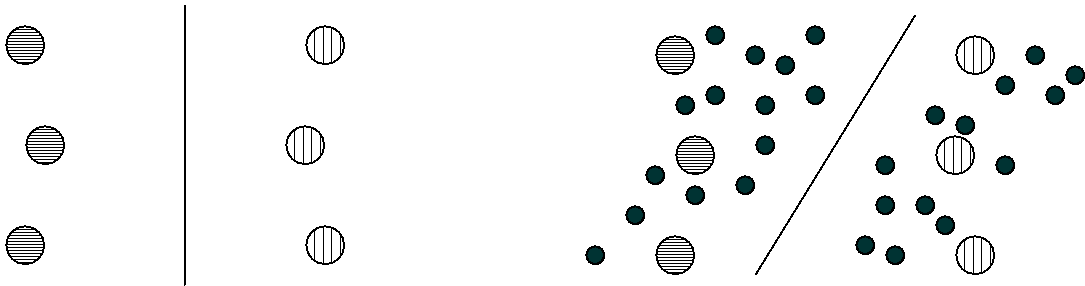
\includegraphics[width=0.5\textwidth]{graphics/s3vm.png}
\begin{tiny}
\caption{ Difference between decision boundary created using only training dataset (left) and pushed boundary by adding unlabeled points (right).\label{fig:SvmMethodFig}}
\end{tiny}
\vspace{1cm}
\end{figure}

\subsection{Graph based method}

One more category of classification methods in semi-supervised learning uses graph representation of the data. In graph based methods of semi-supervised learning, in order to classify the data we create an undirected graph $ G = (V, E) $. The set of nodes $ V $ contains both labeled and unlabeled instances. Edges of the graph, the set $ E $, is representing similarity between two connecting nodes, which can be expressed as weight $ w_{ij} $ between two vertices $x_{i} \text{ and } x_{j} $. Learning using graph methods involves assigning labels $ y $ to each node of the graph by examining the weights. Thanks to the smoothness assumption we might assume that if weight $ w_{ij} $ is large, then two labels $ y_i \text{ and } y_j $ will be the same. Since we have provided small training data, there are nodes already having labels assigned, therefore we are able to classify all nodes in the graph\cite{Zhu06semi}.

Many of the methods for building graphs and estimating weights are distance based, such as fully connected graph, kNN and $\epsilon$NN graphs\cite{Zhu06semi}. In fully connected graph we create edges between all pairs of vertices and we assign weights that are inversely proportional to the Euclidean distance between the nodes. Missing edge would represent an infinite weight\cite{chapelle06}. In kNN case, we only connect k nearest neighbors. $\epsilon$NN takes into account only pairs vertices $ x_i \text{ and } x_j $ with distance $ \| x_i - x_j \| < \epsilon $.\\[1cm]

\begin{figure}[htbp]
\centering
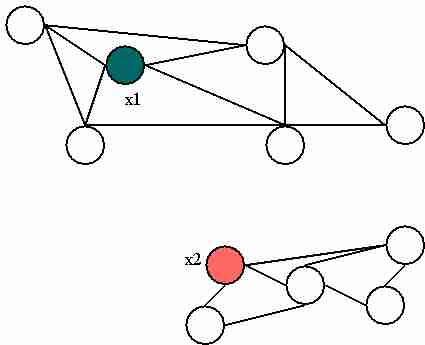
\includegraphics[width=0.3\textwidth]{graphics/graph-methods.jpg}
\begin{tiny}
\caption{ An illustration of how graph based method works.\label{fig:GraphMethodFig}}
\end{tiny}
\vspace{1cm}
\end{figure}

In \emph{Figure~\ref{fig:GraphMethodFig}} we can see a very simplified example in which only two instances $x_1$ and $x_2$ were labeled--- nodes were constructed between nearest neighbors and we can classify those unlabeled by following paths from the labeled data points.

In contrast to distance based methods of building graphs, there are also proposed generative approaches that are claimed to be more effective for certain datasets than methods using discriminative approach\cite{He07}. Rather than calculating Euclidean distance, we estimate conditional probabilities of classes given data points and set them as weights between nodes.

\section{Applications of semi-supervised learning}

Semi-supervised learning has got various applications in real life. It became particularly popular in 1990s when it proved to be useful technique in text classification and natural language processing\cite{chapelle06}. 

Moreover, thanks to relatively good SSL performance we can generalize that it is particularly helpful when the cost of providing labeled training samples is high, such as speech recognition, website classification or even analysis of 3D models of proteins. In bioinformatics applications of TVMs prove to be better than SVMs, however in certain cases they tend to be considerably slower\cite{chapelle06}.
 
Another example is SSL in image processing. It can be applied in consumer applications, such as software for organizing pictures. While in research laboratory it could be possible to label a large dataset, it is not feasible in a typical user environment and SSL can offer good results in labeling images with small training set available\cite{Guillaumin10}.


\chapter{The experiment}

% \section{Sub-Abstract}
\begin{chapabstract}
For experimental part of this assignment we decided to build a simple \emph{self-training semi-supervised} classifier using algorithms already implemented in \texttt{WEKA} machine learning package. The goal is to learn a model from small subset $A$ of training set $U$ and use all remaining instances $B = U \setminus A$ with removed ground truth $B^{\prime}$ to boost it. With such a classifier we want to check whether it will outperform supervised classifier trained only on initial set $A$ and compare it with supervised classifier trained on whole set $U$. The measure of classifiers performance used to evaluate results is a number of correctly classified instances out of whole test set.
% (Confusions Matrices are also provided).
\end{chapabstract}

\section{Background}
As described, the motivation of this project is wide demand for machine learning algorithms which would perform comparably good to supervised learning approaches but require only small fraction of labeled data used with nowadays solutions. The goal of building elementary semi-supervised algorithm is to check whether with simplistic approach we can achieve correct prediction ratio close to the one of some more complex approaches listed in \textbf{Chapter~\ref{ch:sstheory}}. 
%Finally we will propose solution that uses cutting-edge mathematical result which base on \emph{Thompson Sampling} together with \emph{Multi-armed Bandit Theory}.
% Despite the demand in environments where labeling the data is expensive .

\section{Introduction}
Our approach is based on four supervised learning algorithm. We assume that it is more probable that predicted class agrees with ground truth for particular instances if 4 different classifiers agree on predicted label. Following this lead, we compare mentioned statistics of instances and use data points with appended predicted labels to rebuild training set. For comprehensive view multiple sets and approaches are used. In literature such solution is called \emph{self-training algorithm} and number of classifiers that agree on prediction can be considered as \emph{confidence measure}~\cite{zhu2009introduction}. Such algorithms are known to be good in natural language processing but we need to bear in mind that potential error made on predicted label can reinforce itself. We chose this approach as it is the most general one and does not assume any particular distribution within the data. \emph{Self-training} belongs to \emph{wrapper} methods family as it can be used with any approach that measures how good the prediction of unlabeled data is probable to overlap with ground truth.

\section{Experiment design}
% \subsection{General approach}
As explained in \textbf{Chapter~\ref{ch:sstheory}} semi-supervised learning aims at building a classifier from relatively small subset of data which is labeled. To achieve this, we first randomly extract specified number of labeled data points and use them to initially train base classifier. The same sample is used later to train one of supervised classification method to produce predictions that will be used as a \emph{lower bound} on performance (we will call it \emph{supervised classifier trained on initial sample}).

\subsubsection{Remark: Obtaining predictions}
To avoid methodological bias and produce \emph{confidence measure} we decided to use 4 supervised algorithms implemented in \texttt{WEKA}:
\begin{description}
\item[J48 tree] \emph{C4.5 decision tree}--- confidence factor 0.25; the minimum number of objects in the leaf nodes 2; number of folds 3,
\item[IBk] \emph{$k$ nearest neighbors}--- $k$ value equal to 1; linear nearest neighbor search with euclidean distance,
\item[SMO with Polynomial kernel] \emph{sequential minimal optimization algorithm for training a support vector classifier}--- with Polynomial kernel exponent 1,
\item[SMO with RBF kernel] \emph{sequential minimal optimization algorithm for training a support vector classifier}--- with Gamma value 0.01.
\end{description}

The next step is boosting procedure. To this end, the remaining unlabeled instances ($B^{\prime}$) are classified using 4 mentioned algorithms and partitioned into 4 groups which represent \emph{confidence measure} in our approach. Groups are formed according to obtained predictions:\\[-0.6cm]
\begin{center}\textbf{How many classifiers agreed on a prediction:}\end{center}
\begin{tabular}{rp{12cm}}
% \multicolumn{2}{c}{\textbf{How many classifiers agreed on a prediction:}}\\
\textbf{All ($4/4$)} & All 4 \texttt{WEKA} classifiers agreed on one label prediction.\\
\textbf{3 out of 4 ($3/4$)} & 3 classifiers agreed with predicted label. Majority label is selected.\\
\textbf{2 out of 4 ($2/4$)} & 2 classifiers agreed on common label. In case 2 other classifiers have different predicted labels the one of first pair is chosen. On contrary, if other two classifiers have also a common prediction a ``fair coin is tossed'' to select one of them.\\
\textbf{None ($1/4$)} & All classifiers predicted different label. One label is chosen at random.\\[0.4cm]
\end{tabular}

While running the experiment it is possible to decide how many instances from the above categories should be used for boosting procedure. Selected exemplars are labeled based on listed above rules and appended to training set. Then, the remaining unlabeled instances are predicted using re-trained on just expanded set classifiers and grouped again. This process is repeated until person running the experiment decides to stop boosting procedure.\\

Final step is to indicate whether testing will be performed on external test set or on already supplied training set. 
In later case performance of:
\begin{itemize}
\item ``supervised learning'' part of experiment trained on a whole supplied training set is evaluated with \emph{10-folds cross-validation} (``upper bound'');
\item ``supervised learning'' trained only on initial part of training set ($A$) is evaluated on whole set ($U$) and determines a ``lower bound'';
\item semi-supervised learning is evaluated using test set $U$--- the one containing ground truth of each instance.
\end{itemize}

It is also possible to specify a number of testing rounds in case there is no separate test set. In this case two supervised parts of experiment are repeated specified number of times and results for each iteration are summed into global score. For semi-supervised learning results are just multiplied by the number of iterations what results in the same total number of instances to predict throughout all methods to make comparing and contrasting easier.\\

The output of a script consists of confusion matrices and a number of correct predictions for each part of the experiment listed above. The later values are calculated as trace of contingency tables and total number of instances in a data set.

\subsubsection{Remark: Code design and execution of experiment}
To get more details about input, output and usage of the program please follow to \textbf{Appendix~A} or find \texttt{README.md} in GitHub repository~\cite{githubcode}.

\section{The experiment}
To make tests more diverse we decided to use one dataset from each of given below categories:
\begin{itemize}
\item single binary target label,
\item single multivariate target label,% beyond binary classification - multivalued
\item multiple binary valued labels.
% \item multiple multivalued target labels. % if time allows
\end{itemize}
For multi-label data sets the classification is performed separately for each target label and score is calculated as a sum over all labels.\\
By designed interactive nature of the experiment allows multiple configurations for each data set to be tested. What is more, fixing the parameters of a tests up front is not possible as there is an element of randomness in choosing training instances. Therefore, instead of fixing parameters we list the rules to follow in each test in \textbf{Section~\ref{sec:experimetnapproach}}.

\subsection{Used data sets}
Data sets that were used are listed below and respectively match categories given above. To create test and training for \texttt{mushrooms} and \texttt{nursery} the data was shuffled and split in half to create two disjunctive sets from only one provided. \texttt{scene} was already given with separate test and training sets.
\begin{itemize}
\item \texttt{mushrooms}--- Mushrooms Database~\cite{mushroomsDS},
\item \texttt{nursery}--- Nursery Data Set~\cite{nurseryDS},
% \item \texttt{birds}--- Birds Database~\cite{birdsDS},
\item \texttt{scene}--- Scene Database~\cite{sceneDS}.
\end{itemize}

\subsection{Approaches to the experiment\label{sec:experimetnapproach}}
To compare performance of designed semi-supervised algorithm we will consider a few approaches and test them on all chosen data sets.\\
It is possible that initial selection of training instances for semi-supervised learning will be very unlucky and consists only of instances with the same label due to random sampling. 
In real-life such situation is not a thread as instances are carefully selected by scientists to be uniformly distributed. 
In our approach the simplest solution to avoid such ``bad luck'' and make sure that supplied exemplars in training set have diverse class distribution could be repeating random training set initialization until instances are ``almost'' uniformly distributed according to their ground truth. Other approach could be to check whether initial training set is diverse and if not sample instances from unlabeled pool asking user (with our design not needed as ground truth is available) for the label until ``sufficient'' diversity is achieved.\\

Assuming that we have resolved problem of distribution in initial training set the next stage is to describe taken approaches:
\begin{enumerate}
\item \texttt{Maximum exploitation}--- during first boosting iteration all $4/4$ and half of $3/4$ instances are added. Next steps are only taken if there are any elements in mentioned groups and instances are added based on rule: append all elements with higher probability ($4/4\rightarrow3/4\rightarrow2/4\rightarrow1/4$) first until none left,
\item \texttt{No exploration}--- append all instances during first boosting round,
\item \texttt{Maximum exploration}--- during first round append all instances from $4/4$ group. Then, in each round add maximum of $1\%$ of initial number of instances in $U$ with priority given to groups with higher rank. Repeat the last step until no instances are left.
\end{enumerate}
Above experiments are conducted with number of instances in initial training set containing $0.25\%\text{, } 10\% \text{ and } 25\%$ of whole training set ($U$) volume.

\subsubsection{Remark: Initial step}
Number of instances appended to training set during first boosting round seems very important. Reasonably the potential error in prediction of labels that could occur will be reinforced during next iterations of boosting procedure. Potential solution could be maximizing the number of instances added in the first round of boosting as we know that their labels were predicted using classifier trained on a set with correct ground truth. The key point here is to find equilibrium in number of exemplars added in first boosting round to avoid reproducing potential error and do not loose possible information gain in next iterations of semi-supervised model (if we use all instances in first round).
% Give results as snippets on GitHub.
%  are correct so produced classifier will not have any bias due to incorrect training set

\section{Results~\cite{results} \label{sec:results}}
This section will be divided into subsections each corresponding to experiment involving given percentage of initial training set size. Further discussion comparing each of the data sets and taken approach will be included in order depending on outcomes of particular experiment.\\

The experiments with \texttt{scene} data set are only conducted with $0.25\%$ sample size and are presented in \textbf{Section~\ref{sec:results025}}. This decision is due to focus put on very small training sets were we can take full advantage of semi-supervised learning.

\subsubsection{Remark: How to read figures}
In the following three figures: \textbf{\ref{img:25pc}}, \textbf{\ref{img:10pc}} and \textbf{\ref{img:025pc}} percentage of correctly classified instances is shown on y-axis. x-axis ranging from $1$ to $9$ is experiment ID.\\
$x$ in range 1--3 are three results for \texttt{maximum exploitation} approach, 4--6 are outcomes of \texttt{no exploration} and \texttt{maximum exploration} is placed on figures between 7 and 9.\\
\texttt{red} color corresponds to \texttt{mushrooms} data set; \texttt{green} and \texttt{blue} are respectively \texttt{nursery} and \texttt{scene}.\\
Solid \texttt{line} is ``upper bound'' that resulted in training classifier on whole data set. \texttt{\textbf{+}} indicates outcome of semi-supervised learning; finally, \texttt{\textbf{o}} points result of supervised learning only on initial sample of training set.

\subsection{$\mathbf{25\%}$ sample~\cite{results25} \label{sec:results25}}
We will first discuss results with initial sample of size $25\%$ of original training set. The input and output for each of given results are provided together with this report (see references in headers).
\begin{figure}[htbp]
\centering
  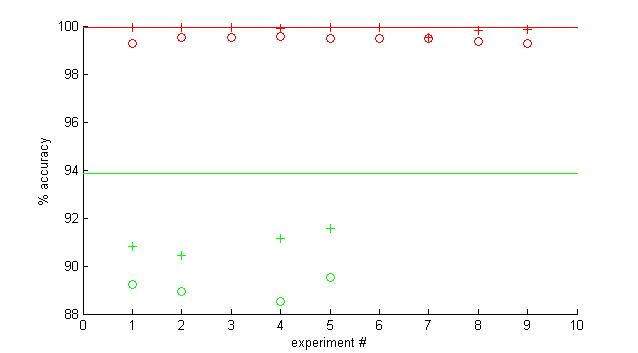
\includegraphics[width=0.5\textwidth]{graphics/figures/Pfig1.jpg}
\begin{tiny}
\caption{\small Figure for $25\%$ sample of volume of initial training set.\label{img:25pc}}
\end{tiny}
\end{figure}

\subsubsection{\texttt{mushrooms}--- \texttt{red}}
Analysis of the outcomes in \emph{Figure~\ref{img:25pc}} gives that performance of semi-supervised algorithm is negligibly better than the one of supervised learning trained on initial sample. Moreover, both these results are not worse than 1\% in comparison with the outcome of supervised classifier trained on the whole set.

\subsubsection{\texttt{nursery}--- \texttt{green}}
In this case semi-supervised learning performs not more than 3\% better than supervised one trained on the same initial sample. We can safely assume that similarly to above example the difference is not significant while considering needed resources.

\subsection*{}
While comparing three taken approaches there is not much difference visible. All of them behave comparably well on sample training size of 0.25 of initial set.\\

Generally, with training set of this size we concluded that performing semi-supervised learning is not worth the time and computational power it takes in comparison with possible accuracy gain. This conclusion is based on outcomes for both data sets as loose in performance do not exceed 3\% while comparing supervised and semi-supervised learning with exactly the same initial training set supplied.\\
In all cases the correct predictions ratio exceeds 88\% what seems quite a good result.

\subsection{$\mathbf{10\%}$ sample~\cite{results10}\label{sec:results10}}
The following figure shows the results of experiment conducted on initial sample of $10\%$ of the training set. The overall outcomes are similar to one presented in \textbf{Section~\ref{sec:results25}}. Nonetheless, we can see minor decrease in performance probably due to more than 2 times smaller training set.

\begin{figure}[htbp]
\centering
  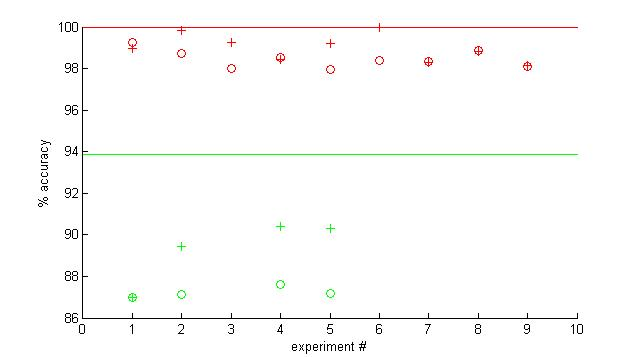
\includegraphics[width=0.5\textwidth]{graphics/figures/Pfig2.jpg}
\begin{tiny}
\caption{\small Figure for $10\%$ sample of volume of initial training set.\label{img:10pc}}
\end{tiny}
\end{figure}

\subsubsection{\texttt{mushrooms}--- \texttt{red}}
The performance of semi-supervised learning on this data set is generally better than outcomes of supervised learning on initial training set. Nonetheless, the difference in accuracy does not exceed 1\% what once again indicates that expensive semi-supervised classification may not be worth the possible gain in number of correct prediction.

\subsubsection{\texttt{nursery}--- \texttt{green}}
Here, outcomes follow similar pattern to the one observed in the example above. Performance of semi-supervised algorithm is persistently better than what can be achieved using supervised learning on initial training sample. The difference in accuracy based on provided outcomes is not more than 3\% what leads to conclusion that also in case of 10\% sample it might not be worth to use proposed semi-supervised algorithm.

\subsection*{}
While comparing the results with regard to used approaches we can clearly see that \texttt{maximum exploitation} ($x \in \left \{ 1, 2, 3 \right \}$) and \texttt{no exploration} ($x \in \left \{ 4, 5, 6 \right \}$) perform better than \texttt{maximum exploration} ($x \in \left \{ 7, 8, 9 \right \}$). In the later one we can see that the results are approximately the same for supervised method trained on initial sample and for semi-supervised algorithm. This observation same as considered complexity of the method leads to conclusion that using the last approach is not worth needed resources.\\

All in all, for 10\% sampling on training set we arrive at similar conclusion that was made in \textbf{Section~\ref{sec:results25}}. Semi-supervised learning gives little improvement over supervised learning algorithm trained on initial sample. Once again possible gain in accuracy, which does not exceed 3\% may not be worth complicated classification procedures.\\
Also here the correct predictions ratio does not drop below 86\% what seems reasonably good outcome.


\subsection{$\mathbf{0.25\%}$ sample~\cite{results025}\label{sec:results025}}
For 0.25\% sampling of initial training set we arrive at \emph{Figure~\ref{img:025pc}} presented below. In this case the training set contains around 10 instances whereas full set has above 4000 exemplars. With such a small training set we can spot advantages of proposed algorithm over supervised learning on initial training set. The gap in accuracy between semi-supervised and supervised algorithm trained on initial sample increased to maximum of 15\%. The later result gives possibility of improving classification process by using proposed here algorithm in cases where only a very small amount of labeled data is available.

\begin{figure}[htbp]
\centering
  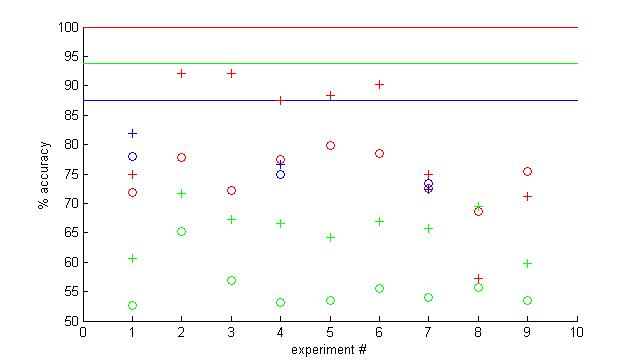
\includegraphics[width=0.5\textwidth]{graphics/figures/Pfig3.jpg}
\begin{tiny}
\caption{\small Figure for $0.25\%$ sample of volume of initial training set.\label{img:025pc}}
\end{tiny}
\end{figure}

\subsubsection{\texttt{mushrooms}--- \texttt{red}}
The experiments on this data set prove increase in accuracy while using semi-supervised learning. First two approaches ($x \in \left \{ 1, 2, 3 ,4, 5, 6 \right \}$) perform significantly better (15\% on average) than the last one. Moreover, number of correct prediction is only 7\% less in semi-supervised learning than in supervised one trained on whole set.

\subsubsection{\texttt{nursery}--- \texttt{green}}
Improvement in semi-supervised learning seems to be consistent through all experiments being on average 10\% in terms of number of correct prediction. Even though the results seem to be advantageous for semi-supervised learning the best achieved accuracy is about 20\% worse than the one achieved with supervised learning trained on whole set.

\subsubsection{\texttt{scene}--- \texttt{blue}}
Designed algorithm seems to give only little improvement on multi-labeled data sets. Here, the increase in accuracy does not exceed 5\%. Moreover, the results of semi-supervised learning are on average 10\% worse than number of correct predictions achieved with classifier trained on whole data set. This result seems interesting and needs further investigation as either treating labels independently or having unbalanced class distribution have detrimental effect on designed algorithm in comparison with other used data sets.

\subsection*{}
Once again we can spot the advantage of first two proposed approaches ($x \in \left [ 1,6   \right ] $) over the third one. Moreover, first one seems to perform slightly better than the other. We can conclude that boosting training set with very small data samples is detrimental to designed algorithm and the focus should be put on first two approaches. This effect can be easily seen within \texttt{mushrooms} data set and it also has slight effect on \texttt{scene} but is not present in \texttt{nursery}. This observation results in conclusion that the last approach is not consistent throughout data set and should be neglected in further discussions.\\

In two previous experiments with initial training size of 25\% and 10\% volume we could state without any doubts that achieved improvement while using semi-supervised learning is not worth its effort. On contrary, here the improvement is significant and both approaches used are relatively simple.\\
In \texttt{mushrooms} and \texttt{scene} data set the performance is about 7\% worse than the one achieved with full training set. In \texttt{nursery} this value oscillates around 20\%.\\
To sum up, the improvement with semi-supervised learning reaches 15\% while in general the worse performance of proposed algorithm does not drop below 60\%.



\subsection{Data sets overview}
\emph{Figures~\ref{img:mushrooms},~\ref{img:nursery},~\ref{img:scene}} presented below are showing outcomes of \texttt{mushrooms}, \texttt{nursery} and \texttt{scene} data sets respectively. y-axis contains number of correctly classified instances and x-axis is the ID of the experiment in the same order as in previous figures.\\
Magenta solid line represents the total number of exemplars. Blue solid line is the number of correctly classified instances while using supervised algorithm trained on whole training set. Colors: red, green and blue corresponds to 25\%, 10\% and 0.25\% samples accordingly. \texttt{\textbf{+}} symbol indicates outcome of semi-supervised algorithm while, \texttt{\textbf{o}} illustrates the same value for supervised algorithm trained only on initial sample.\\

\begin{figure}[htbp]
	\centering
	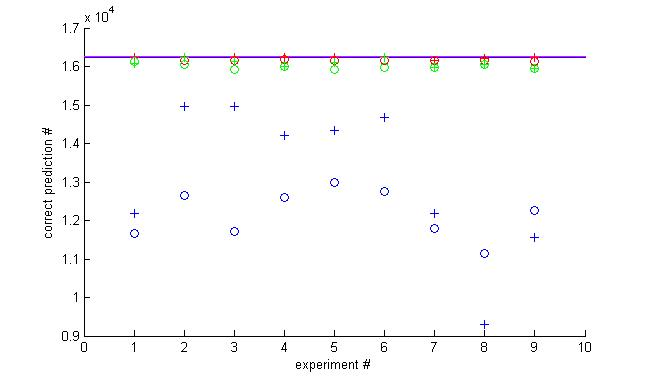
\includegraphics[width=0.5\textwidth]{graphics/figures/fig1.jpg}
	\begin{tiny}
		\caption{\small \texttt{mushrooms} data set.\label{img:mushrooms}}
	\end{tiny}
\end{figure}
\texttt{mushrooms} (\emph{Figure~\ref{img:mushrooms}}) data set will be considered first. For both 25\% and 10\% sample the results are very similar and the difference does not seem important with regard to proposed semi-supervised algorithm. Classification on 0.25\% sample seems consistent and effective through first two approaches and gives significant improvement with described algorithm while with third approach it seems to fail. With regard to this set we can claim that desired goal has been achieved.\\


\begin{figure}[htbp]
	\centering
	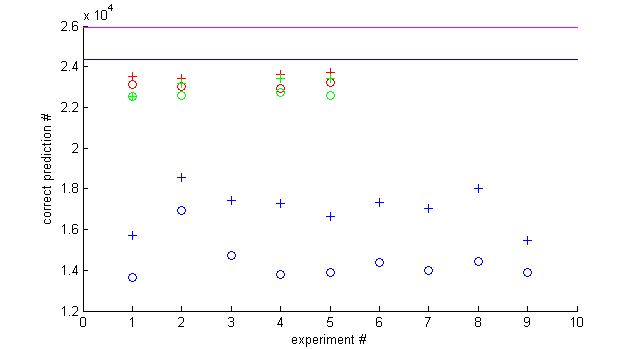
\includegraphics[width=0.5\textwidth]{graphics/figures/fig2.jpg}
	\begin{tiny}
		\caption{\small \texttt{nursery} data set.\label{img:nursery}}
	\end{tiny}
\end{figure}

\texttt{nursery} (\emph{Figure~\ref{img:nursery}}) gives consistent results for all approaches. For samples of size 25\% and 10\% the number of correct predictions is relatively high for both semi-supervised learning and supervised learning on initial sample what leads to conclusion that first one is not worth performing same as in \texttt{mushrooms}. On contrary, in 0.25\% sample we get very good improvement while using designed algorithm.\\

\begin{figure}[htbp]
	\centering
	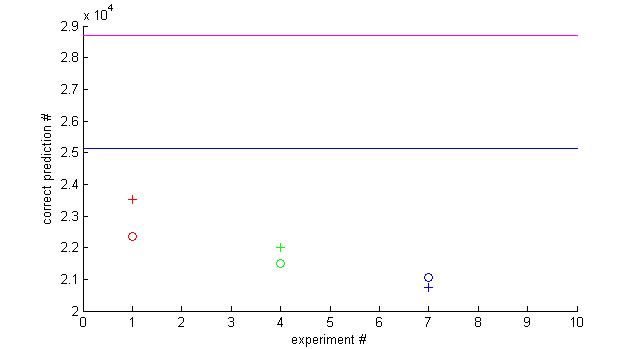
\includegraphics[width=0.5\textwidth]{graphics/figures/fig3.jpg}
	\begin{tiny}
		\caption{\small \texttt{scene} data set.\label{img:scene}}
	\end{tiny}
\end{figure}

Third one--- \texttt{scene} (\emph{Figure~\ref{img:scene}}) which represents multi-label data set is not much of a help in our experiment. Achieved improvement in semi-supervised learning seems relatively low in comparison with two other datasets. Nonetheless, the results of this trial confirm the general conclusions that \emph{first approach}--- \texttt{maximum exploitation} is the best one proposed giving highest overall improvement in semi-supervised learning over supervised learning trained on initial sample.\\


\section{Conclusions}
To sum up, using designed and tested by us classifier can not harm the classification what was shown in \textbf{Section~\ref{sec:results}}.
First two approaches seems stabel and give overall improvement in all data sets while the last one does not always  give better accuracy.
% \section{More complex solution} \lipsum[1]


\clearpage
\newpage
\section*{Appendix: A--- Code design\label{ap:code}}
% include morkdown README.md
\include*{readme}

% Then supervised algorithm as predictors
% \newpage
% \begin{center} \vspace*{5cm}\textbf{\huge FIN}\vspace*{5cm} \end{center}

\bibliographystyle{plain}
\bibliography{references}{}

\end{document}
